\section{Specyfikacja techniczna}
\indent Główna aplikacja opracowana zostanie przy użyciu środowiska Microsoft Visual Studio. Do implementacji głównej aplikacji zawierającej zaimplementowany algorytm genetyczny i interfejs użytkownika wykorzystane zostaną podstawowe biblioteki standardowe dostępne w środowisku Visual Studio. \newline
\indent Narzędziem dodatkowo wspomagającym opracowywanie oprogramowania systemu jest system kontroli wersji GIT - GitHub. \newline
\indent Sterownik PLC wykorzystywany do zrealizowania omawianego systemu to moduł S7-1200 firmy Siemens. Komunikacja pomiędzy stacją operatorską (PC, tablet, laptop) a sterownikiem PLC realizowana będzie przy użyciu sieci Ethernet.\newline
\indent Kluczowe elementy omawianego systemu przedstawiono na wcześniej zamieszczonych diagramach UML.Poniżej umieszczono diagram UML ukazujący interakcje pomiędzy składowymi elementami oprogramowania.
\begin{figure}[ht!]
\centering
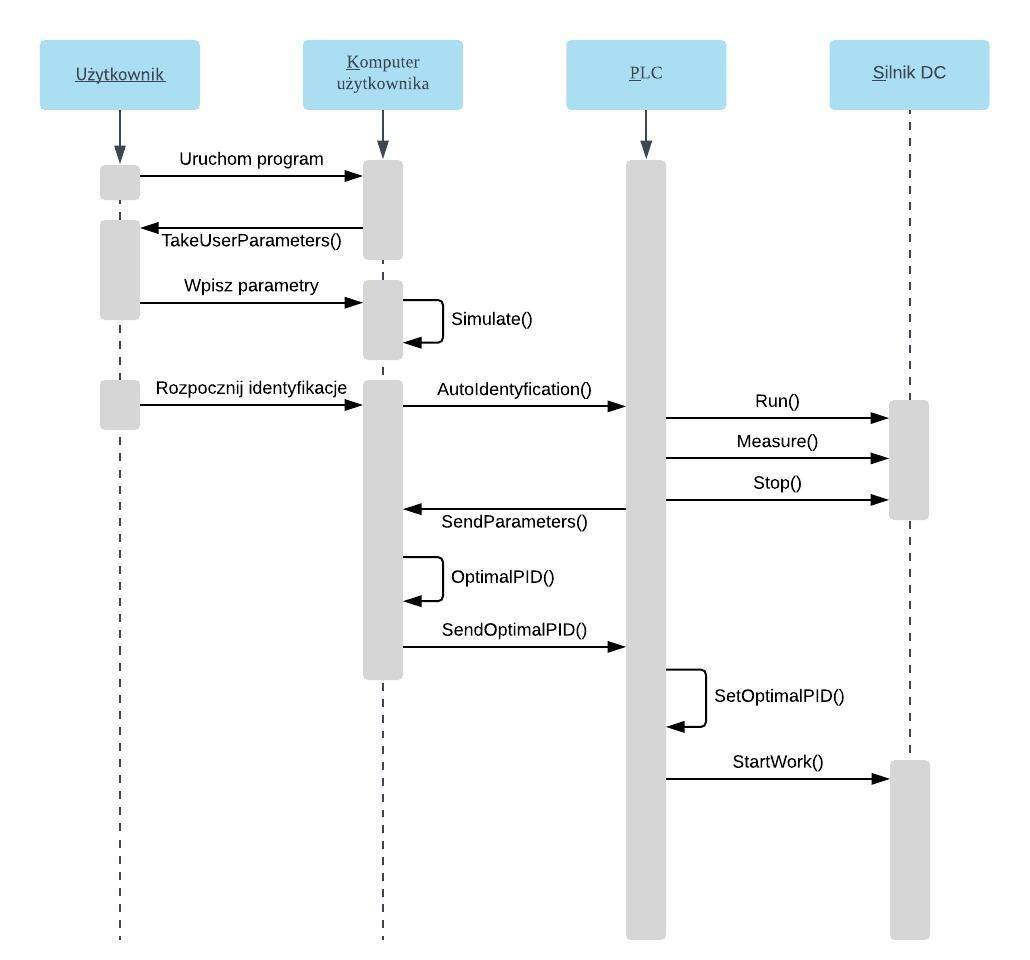
\includegraphics[scale=0.42]{uml}
\caption{Diagram UML przedstawiający interakcje pomiędzy składowymi oprogramowania i systemu}
\label{komponent2}
\end{figure} 
\newpage
\subsection{Harmonogram i podział pracy}
\begin{table}[ht]
	  \caption{Harmonogram prac związanych z realizacją projektu}
    \begin{tabular}{|c|c|l|}
    \hline
    \multicolumn{1}{|c|}{Lp.} & \multicolumn{1}{c|}{Data zakończenia zadań} & \multicolumn{1}{c|}{Zadania do zrealizowania} \\
    \hline
       1.  &16.05.2018 & \begin{tabular}{  L{0.55\textwidth}  m{0.45\textwidth} | }1. Określenie użytkowników końcowych systemu, na podstawie rozmów z klientem.\\2. Zdefiniowanie wymagań funkcjonalnych i pozafunkcjonalnych dla opracowywanego systemu.\\3. Opracowanie dokumentacji funkcjonalnej, zawierającej powyższe informacje oraz scenariusz użycia systemu i odpowiednie diagramy UML. \\ 4. Prezentacja aktualnych efektów prac nad projektem przed docelowym klientem.\end{tabular} \\
    \hline
       2.  &23.05.2018 & \begin{tabular}{  L{0.55\textwidth}  m{0.45\textwidth} | } 1. Utworzenie oraz odpowiednia organizacja repozytorium projektu w serwisie GitHub.com.\\ 2. Wybór języka programowania, środowiska IDE, bibliotek zastosowanych do opracowania oprogramowania.\\ 3. Opracowanie specyfikacji technicznej zawierającej m.in. modele UML kluczowych elementów systemu. \\ 4. Prezentacja aktualnych efektów prac nad projektem przed docelowym klientem. \\ \end{tabular} \\
    \hline
       3.  &06.06.2018  &  \begin{tabular}{  L{0.55\textwidth}  m{0.45\textwidth} | } 1. Opracowanie modelu matematycznego silnika DC. \\
       2. Rozpoczęcie opracowywania oprogramowania aplikacji i jej interfejsu graficznego.\\ 3. Rozpoczęcie implementacji optymalizatora nastaw i komunikacji z PLC. \\ 4. Opracowanie dokumentacji wykonanych prac. 5. Konsultacja otrzymanych wyników prac z docelowym klientem. \\ \end{tabular} \\
    \hline
       4.  & 13.06.2018      & \begin{tabular}{  L{0.55\textwidth}  m{0.45\textwidth} | } 1. Wykonanie odpowiednich cykli testów jednostkowych oprogramowania. \\2. Profilowanie aplikacji i próba optymalizacji hot spotów.\\ 3. Odpowiednie udokumentowanie przebiegu wykonywanych testów.\\ 4. Przedstawienie klientowi dotychczasowych wyników i wykonanie ewentualnych poprawek.\\ \end{tabular} \\
    \hline
       5.  & 30.06.2018     & \begin{tabular}{  L{0.55\textwidth}  m{0.45\textwidth} | } 1. Implementacja aplikacji na rzeczywistym obiekcie.\\ 2. Wykonanie serii testów działania systemu w warunkach docelowych. \\ 3. Naniesienie poprawek do oprogramowania systemu i ich dokumentacja.\\4. Oddanie systemu do użytku klienta.\\ \end{tabular} \\
    \hline
    \end{tabular}
  \label{tabelka}
\end{table}
\indent Realizacja omawianego systemu, którego charakterystykę i opis przedstawiono w niniejszym opracowaniu wymaga odpowiedniego zaplanowania prac zespołu, które umożliwią zakończenie całego projektu sukcesem. Harmonogram prac związanych z opracowaniem oprogramowania i realizacją całości systemu przedstawiono w tabeli \ref{tabelka} znajdującej się na następnej stronie.
	


\indent Na podstawie zdefiniowanych wymagań dotyczących funkcjonalności systemu zdefiniowano następujący podział pracy w zespole:
\vspace{0.3cm}
\begin{itemize}
\item \textbf{Kamil Andrzejewski} - prowadzenie porządku w repozytorium - GIT maintainer, komunikacja PLC
\item \textbf{Maciej Zielonka} - implementacja algorytmu genetycznego, implementacja aplikacji optymalizującej
\item \textbf{Paweł Zarembski} - zaprojektowanie i implementacja interfejsu użytkownika
\item \textbf{Paweł Spławski} - tworzenie dokumentacji projektu, opracowanie modelu silnika DC
\end{itemize}
